\documentclass{article}

\usepackage{hyperref}
\usepackage{enumerate}
\usepackage{enumitem}
\usepackage{amssymb,amsmath,amsthm} %must be before unicode-math
\usepackage[mathletters]{ucs}
\DeclareUnicodeCharacter{8348}{_t}
\DeclareUnicodeCharacter{8342}{_k}
\DeclareUnicodeCharacter{8339}{_x}
\DeclareUnicodeCharacter{8345}{_n}
\DeclareUnicodeCharacter{7522}{_i}
\DeclareUnicodeCharacter{11388}{_j}
\DeclareUnicodeCharacter{7523}{_r}
\DeclareUnicodeCharacter{7580}{^c}
\DeclareUnicodeCharacter{7496}{^d}
\DeclareUnicodeCharacter{7511}{^t}

\usepackage[utf8x]{inputenc}
\usepackage{graphicx}
\usepackage{stmaryrd}
\usepackage[autosize]{dot2texi}
\usepackage{multicol}
\setlength{\multicolsep}{0pt}
\usepackage{tikz}
\usetikzlibrary{shapes,arrows,tikzmark,decorations.pathreplacing,calc}
\usepackage{adjustbox}

% Title portion. Note the short title for running heads
\title{Solving smooth system of algebraic equations}
\author{Christophe Raffalli}

\newcommand{\interior}[1]{%
  #1^{\mathrm{o}}%
}
\newcommand{\cardinal}[1]{%
  \#({#1})%
}
\newcommand{\hull}[1]{%
  \mathcal H({#1})%
}
\newcommand{\cone}[1]{%
  \mathcal C({#1})%
}
\newcommand{\vertices}[1]{%
  \mathcal V({#1})%
}
\newcommand{\ball}[2]{%
  \mathcal B_{#2}({#1})%
}

\newcommand{\PNR}{{\cal P}^n(ℝ)}
\newcommand{\SNR}{{\cal S}^n(ℝ)}

\newtheorem{theo}{Theorem}
\newtheorem{nota}[theo]{Notation}
\newtheorem{defi}[theo]{Definition}
\newtheorem{prop}[theo]{Proposition}
\newtheorem{exam}[theo]{Example}

% Document starts
\begin{document}


\maketitle

\section{Introduction}

\begin{figure}
  \begin{center}
    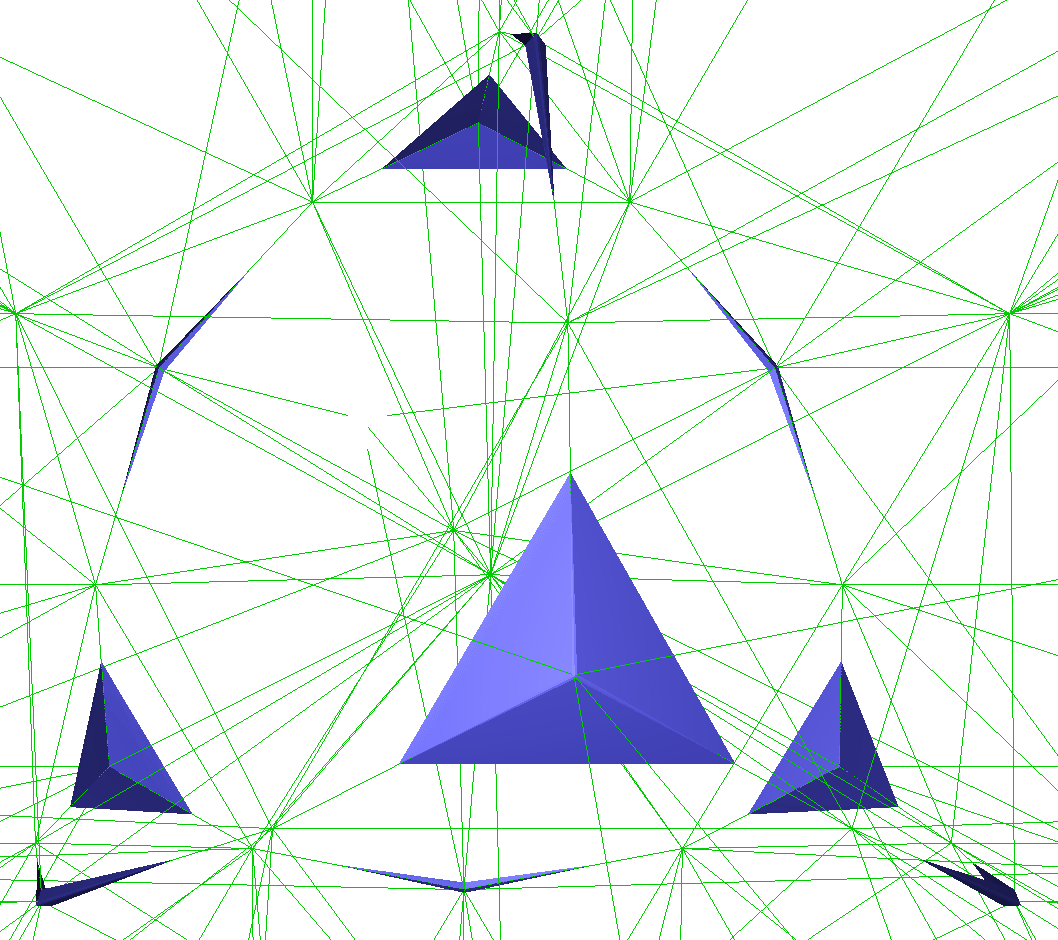
\includegraphics[width=\linewidth]{quartic-M-2.png}
    \caption{piecewise linear approximation of a quartic surface}
  \end{center}
\end{figure}

We present an algorithm solving smooth systems of homogeneous polynomial
equations $\{x ∈ \PNR, p₁(x) = 0, \dots, pₖ(x) = 0\}$. By \emph{smotth},
we mean than the vectors $(∇p₁(x),\dots,∇pₖ(x))$ are linearly independant for
all $x$. By
\emph{solving} we mean finding a piecewise linear approximation of the
solution that is homeomorphic to the real solution allowing for instance to
compute topological invariants of the solution and in particular the number of
connected components. We therefore do not limit ourselves to the zero
dimensional case.

To obtain the solution, we partition the projective space $\PNR$ is a
family of simplices $(Δⱼ)_{j∈J}$, then we construct
the piecewise linear functions $\overline{p}ᵢ$ that are linear on each $Δⱼ$ and
coincide with $pᵢ$ on the vertices of the simplices $Δⱼ$.

Then, we give a criteria to ensure that the set $\{x ∈ \PNR,
\overline{p}₁(x) = 0, \dots, \overline{p}ₖ(x) = 0\}$ is homeomorphic to the
solution of the original system.

The criteria can be summarised as follows:
\begin{itemize}
  \item For each point $x$ of $\PNR$, consider the set of simplices $\{Δ_{j₁},
    \dots, Δ_{jₘ}\} = \{Δⱼ, x ∈ Δⱼ\}$.
  \item For each polynomial $pᵢ$, this gives a set of $m+1$ vector: the gradient
    of the original polynomial $pᵢ$ at $x$, and the gradient of each linear
    function ${\overline{p}ᵢ}_{\restriction Δ_{jₖ}}$ at $x$:
    $$Gᵢ(x) = \{∇pᵢ(x),∇{\overline{p}ᵢ}_{\restriction Δ_{j₁}}(x),  \dots,
      ∇{\overline{p}ᵢ}_{\restriction Δ_{jₘ}}(x)\}$$
    \item Then the criteria is satisfied if for any $x \in \PNR$ such that ...
      and for any
      $(ε₁,\dots,εₖ) ∈ \{-,+\}ᵏ$, $0$ is not in the convex hull of
      $ε₁ G₁(x) ∪ \dots ∪ εₖ Gₖ(x) $.
\end{itemize}

This gives the spirit of the criterion. The real criterion needs a bit more care
as gradient of polynomials are not well defined
This criteria can be checked in practice with a sufficient condition as precise
as we want (up to more computation) using the fact that polynomials written in
the Berstein bases are in the convex hull of their coefficients.

The part of the algorithm is to construct a partition of $\PNR$ that satisfy the
above criterion. We are not yet able to prove that this part of our algorithm
terminates. But it does terminate in practice. It even seem that it requires a
partition whose size is bounded by a constant that only depends upon the number
of variables, number of polynomials and their degree (see conjecture \ref{?}).

Is important to remark that the correction of the algorithm only requires the
criterion to be proved correct, which is done in that paper.

%<!-- Local IspellDict: british -->
%<!-- Local IspellPersDict: ~/.ispell-british -->

\section{Conventions and notations}

We consider the real projective plane $\PNR$.
 We define $πₙ:ℝ^{n+1}∖\{0\} → \PNR$ the
projection $x ↦  \{ λx, λ∈ℝ^⋆ \} ∈ \PNR$. To simplify, we often write $\overline{x}$ for $πₙ(x)$.


We use on $\PNR$ the measure and topology induced by
the chord metric of the unit sphere:
$$d(\overline{x},\overline{y}) = \min\left(
\left\|{\frac{x}{\|x\|}} - {\frac{y}{\|y\|}}\right\|, \left\|{\frac{x}{\|x\|}} + {\frac{y}{\|y\|}}\right\|\right) (∀\overline{x},\overline{y} ∈ \PNR).$$

If $x ∈ \PNR$ (resp. $ℝ^{n+1}$), $\ball{x}{r}$ denotes the open ball of center $x$
and radius $r$ and $\cball{x}{r}$ denotes its closure.

We write $\cardinal{S}$ the cardinal of a set $S$.

For $A ⊂ ℝ^{n+1}$, $\hull{A}$ denotes the convex hull of $A$ and $\cone{A}$ its
convex cone:
$$\cone{A} = \{ ∑_{i=0}ⁿ λᵢ xᵢ, x₀,\dots,xₙ ∈ A, λ₀,\dots,λₙ∈ℝ^⋆₊\}$$
$$\hull{A} = \{ ∑_{i=0}ⁿ λᵢ xᵢ, x₀,\dots,xₙ ∈ A, λ₀,\dots,λₙ∈ℝ^⋆₊,
∑_{i=1}ⁿ λᵢ=1 \}$$

We use the following notation for closed simplices:
\begin{itemize}
\item If $Δ ⊂ \PNR$ is a closed simplex, we denote $\vertices{Δ} ⊂ \SNR$ a finite set of
  representatives of the vertices of $Δ$.
\item $\vertices{Δ}$ must verify that $Δ = πₙ(\hull{\vertices{Δ}})$. This is why we take $\vertices{Δ} ⊂
    \SNR$ instead of $\vertices{Δ} ⊂ \PNR$ as the convex hull is not well defined in
    the projective plane.
\item Simplices should not be too big, in particular, $\PNR$ is not a simplex!
  For this we require $\vertices{Δ}$ to fit in an open half space of
  $\SNR$. If this is not possible, we consider that $Δ$ is not a simplex.
\item We take $\vertices{Δ}$ to be minimal and consider only non degenerated simplex: removing one point in
    $\vertices{Δ}$
    changes it convex hull and the dimension of the
    simplex $Δ$ is always exactly $\cardinal{\vertices{Δ} - 1}$. This also means that
    $\vertices{Δ}$ is the set of extremal points of its convex hull.
  \item Because we require simplices to be not too big $πₙ^{-1}(Δ)$ has exactly two connected components:
    $$πₙ^{-1}(Δ) = \cone{\vertices{Δ}} ∪ -\cone{\vertices{Δ}}.$$
    We write $Δ⁺ =  \cone{\vertices{Δ}}$ and $Δ⁻ = - Δ⁺$. Here $-A$ denotes
    $\{-x, x ∈ A\}$.

\end{itemize}

%<!-- Local IspellDict: british -->
%<!-- Local IspellPersDict: ~/.ispell-british -->

\section{Simplicial partition}

\begin{defi}
  A \emph{simplicial partition} of
  $\PNR$ is a finite set of closed simplices $(Δᵢ)_{i∈I}$ such that
  \begin{itemize}
  \item Each $Δᵢ$ is a simplex of dimension $n$, i.e. $\cardinal{\vertices{Δ}} = n + 1$.
  \item $⋃_{i∈I} Δᵢ = \PNR$,
  \item For all $i₁ < i₂ < \dots iₖ ∈ I$, $Δ_{i₁} ∩ \dots ∩ Δ_{iₖ}$ is empty or is a simplex of dimension at most
    $n-k+1$ and $πₙ(\vertices{Δ_{i₁} ∩ \dots ∩ Δ_{iₖ}}) =
    πₙ(\vertices{Δ_{i₁}}) ∩ \dots ∩ πₙ(\vertices{Δ_{iₖ}})$.
    We can not require  $\vertices{Δᵢ ∩ Δⱼ} = \vertices{Δᵢ} ∩ \vertices{Δⱼ}$ because we may have $x ∈
    \vertices{Δᵢ}$ and $y ∈ \vertices{Δⱼ}$ with $x ≠ y$ and $\overline{x} = \overline{y}$ (see
    the example below). This conditions ensures that the intersection of
    simplices consists exactly in the face of lower dimensions defined by the
    common vertices of the simplices.
%  \item We say that $Δᵢ$ and $Δⱼ$ are neighbour if $Δᵢ ∩ Δⱼ ≠ ∅$. The neighbourhood relation is clearly reflexive and symmetric.
  \end{itemize}
\end{defi}

Here is as example a partition of $\PNR$ with $2ⁿ$ simplices:
\begin{exam}\label{init_part}
Consider $B = \{x₀,\dots,xₙ\}$, the canonical base of $ℝ^{n+1}$ and
$(εᵢ)_{i ∈ \{1,\dots,2ⁿ\}}$ an enumeration of all sequences of length $n$ of
$1$ or $-1$. Then, we define $(Δᵢ)_{i∈\{1,\dots,2ⁿ\}}$ by
$$Δᵢ = πₙ(\hull{\{x₀,ε_{i,1} x₁, \dots, ε_{i,n} xₙ\}}).$$
\end{exam}

We remark in this example, that all simplices use $B$ as set of vertices. This
means that for all $i < j ∈ \{1,\dots,2ⁿ\}$, we have
  $πₙ(\vertices{Δᵢ}) = πₙ(\vertices{Δⱼ}) = πₙ(B)$ while $\vertices{Δᵢ} ≠ \vertices{Δⱼ}$.

In this examples, we have
\begin{eqnarray*}
  Δ⁺ᵢ &=& \cone{\{x₀,ε_{i,1} x₁, \dots, ε_{i,n} xₙ\}} \cr
  Δ⁻ᵢ &=& \cone{\{-x₀,-ε_{i,1} x₁, \dots, -ε_{i,n} xₙ\}} \cr
\end{eqnarray*}

\begin{defi} Let $(Δᵢ)_{i∈I}$ be a simplicial partition of $\PNR$. For $x ∈
  ℝ^{n+1} ∖\{0\}$ we define
  $I^Δ(x) = \{(i,σ) ∈ I × \{-,+\}, x ∈ Δᵢ^σ\}$. In general we only use one
  simplicial partition at a time and we simply write $I(x)$.
\end{defi}

\begin{prop}\label{Ihomo}
  Let $(Δᵢ)_{i∈I}$ be a simplicial partition of $\PNR$.
  For $x ∈  ℝ^{n+1} ∖\{0\}$ and $λ > 0$, we have $I(λx) = I(x)$.
\end{prop}

\begin{proof}
  From the fact that the set $Δᵢ^σ$ are convex cones.
\end{proof}

%<!-- Local IspellDict: british -->
%<!-- Local IspellPersDict: ~/.ispell-british -->

\section{Δ-linear approximation of a polynomial}

\begin{defi}
Let $p$ be an homogeneous polynomial of degree $d$ on
$ℝ^{n+1}$. Let $(Δᵢ)_{i∈I}$ be a simplicial partition of $\PNR$.
We define $\overline{p} : ℝ^{n+1} → ℝ$, the \emph{$Δ$-linear approximation of $p$},
the piecewice linear function
that is linear on all $Δ^σᵢ$ for $i ∈ I$, $σ ∈ \{+,-\}$, and equal to $p$
on all points in $\vertices{Δ}$.

For $i ∈ I$, $σ ∈ \{+,-\}$, we define $∇ᵢ^σp = ∇\overline{p}(x)$
for any $x ∈ Δ^σᵢ$, as the gradient is constant over $Δ^σᵢ$ for a linear
function.

We also define $\hat p(x) = \sgn(\overline{p}(x))^{d-1} \overline{p}^d(x)$. $\hat p$
is homogeneous of degree $d$, i.e. for $x \in ℝ^{n+1}$ and $λ>0$, $\hat p(λx) = λᵈ
\hat p(x)$. The function $\overline{p}$ and $\hat p$ obviously have the same sign and
zero locus on $ℝ^{n+1}$.
\end{defi}

\begin{lemm}
Let $p$ be an homogeneous polynomial of degree $d$ on
$ℝ^{n+1}$. Let $(Δᵢ)_{i∈I}$ be a simplicial partition of $\PNR$.
The function $\overline{p}$ and $\hat p$ have derivatives at $x ∈ ℝ^{n+1} ∖\{0\}$ in the
direction $v$ if the point $I(x + h v)$ is constant
for $h ∈ [-ε,ε]$ with $ε > 0$ is small enough.

This means that for any line segment $\overline{p}$ and $\hat p$ have
derivatives almost everywhere in the direction of this line.
\end{lemm}

\begin{proof}
  Lines can only meet transversaly intersections $πₙ^{-1}$ of the intersection
  of at least two simplices of $Δ$ in finitely many points.
\end{proof}

\begin{lemm}
  From the previous lemma, with the same hypothesis, we find that $\hat p$ is
  Lipschitz in $\ball{0}{M}$ for any $M ∈ ℝ₊$.
\end{lemm}

\begin{proof}
  Let $L$ be the maximum of the differential of $\hat p$, where it is defined in
  $\ball{0}{M}$. At a point $x$ in $D = \ball{0}{M} ∩ πₙ^{-1} (Δ_{i₁} ∩ \dots ∩
  Δ_{iₖ})$, if $v$ is a direction tangent to this intersection, then $\nabla
  \hat p_{i₁}(x) . v = \dots = \nabla \hat p_{iₖ}(x) . v$ because the functions
  $\hat p_{i₁}, \dots, \hat p_{iₖ}$ coincide on $D$. We will denote this number
  by $\nabla \hat p(x) . v$, which for $v$ fixed is defined almost every where,
  and we have $\nabla \hat p(x) . v ≤ \min_{j ∈ (i₁,\dots,iₖ)} \|\nabla \hat
  pⱼ(x)\| \|v\| ≤ L \|v\|$.

  Then, we have
  \begin{eqnarray*}
    |\hat p(x) - \hat p(y)| &=& \left. ∫₀¹ \nabla \hat p(x + (1-t) y) . (x - y)
    dt\right. \cr
    &≤&   ∫₀¹ L \|(x - y)\| dt \cr
    &≤& L \|x - y\|
  \end{eqnarray*}
\end{proof}

\begin{defi}
Let $p$ be an homogeneous polynomial of degree $d$ on
$ℝ^{n+1}$. Let $(Δᵢ)_{i∈I}$ be a simplicial partition of $\PNR$.
Let $\overline{p}$ be the $Δ$-linear approximation of $p$.
We define
\begin{itemize}
  \item the condition $Π_p(x)$ to be true if and only if $p(x)$ and
$\overline{p}(x)$ are both positive or both negative (i.e. $p(x)
    \overline{p}(x) > 0$),
  \item The set $\ncone{p}{x} = \cone{\{∇p(x)\} ∪ \{∇ᵢ^σp, (i,σ) ∈ I(x)\}}$
  \item The set $\nhull{p}{x} = \hull{\{∇p(x)\} ∪ \{∇ᵢ^σp, (i,σ) ∈ I(x)\}}$
\end{itemize}
\end{defi}

\begin{prop}\label{adaptedeq}
Let $p$ be an homogeneous polynomial of degree $d$ on
$ℝ^{n+1}$. Let $(Δᵢ)_{i∈I}$ be a simplicial partition of $\PNR$.
Let $\overline{p}$ be the $Δ$-linear approximation of $p$.

The following conditions are equivalent:
\begin{enumerate}
\item $∀x ∈  ℝ^{n+1}∖\{0\}, Π_p(x) \hbox{ or } 0 ∉ \ncone{p}{x}$
\item $∀x ∈  ℝ^{n+1}∖\{0\}, Π_p(x) \hbox{ or } 0 ∉ \nhull{p}{x}$
\item $∀x ∈  \SNR, Π_p(x) \hbox{ or } 0 ∉ \ncone{p}{x}$
\item $∀x ∈  \SNR, Π_p(x) \hbox{ or } 0 ∉ \nhull{p}{x}$
\item\label{hb} $∀x ∈  ℝ^{n+1}∖\{0\}, Π_p(x) \hbox{ or } ∃δ ∈ ℝ^{n+1}∖\{0\},
  \left\{\begin{array}{l} δ.∇p(x) > 0 \hbox{ and}\cr
    ∀(i,σ) ∈ I(x), δ.∇ᵢ^σp > 0
  \end{array}\right.$
\end{enumerate}
\end{prop}

\begin{proof}
  The equivalences (1) ↔ (2) and (3) ↔ (4) are a general property of convex hull
  and convex cone: for any set $X ⊂ ℝ^{n+1}$, $0 ∈ \hull{X} ↔ 0 ∈ \cone{X}$.
  %Left to right is because $\hull{X} ⊆ \cone{X}$. For right to left, if $0 ∈
  %\cone{X}$, if means we write $0 = λᵢ x₁ + \dots + λₙ xₙ$ with $λᵢ > 0$ and
  %$xᵢ ∈ X$ for $1 < i < n$. Hence, taking $μᵢ = \frac{λᵢ}{λᵢ + \dots + λₙ}$, we
  %have $0 = μᵢ x₁ + \dots + μₙ xₙ$ with $μ₁ + \dots + μₙ = 1$ and $μᵢ > 0$, $xᵢ
  %∈ X$ for $1 < i < n$.


  The equivalence (1)  ↔ (3) comes from proposition $\ref{Ihomo}$ and the fact that $p$ is homogeneous hence
  $\nabla(p)(λx) = λ^{d-1}\nabla(p)(x)$ for $λ > 0$.

  The equivalence (2) ↔ (5) is a form of Han-Banach theorem ensuring the
  existence of a supporting hyper-plane for points outside a convex body. The
  vector $δ$ is a normal vector of this supporting hyperplane \cite{Zal02}.
\end{proof}

\begin{defi}
Let $p$ be an homogeneous polynomial of degree $d$ on
$ℝ^{n+1}$. Let $(Δᵢ)_{i∈I}$ be a simplicial partition of $\PNR$.
We say that the partition is \emph{adapted} to $p$ if it satisfies the conditions
of proposition \ref{adaptedeq}.
\end{defi}

\begin{coro}
  Let $p$ be an homogeneous polynomial of degree $d$ on
  $ℝ^{n+1}$. Let $(Δᵢ)_{i∈I}$ be a simplicial partition of $\PNR$ adapted to $p$.
  Then, the zero-locus of $p$ and $\overline{p}$ the $\Delta$ approximation of
  $p$ are isomorphic.
\end{coro}

This theorem is a consequence of the theorem \ref{maintheo} to come.

\begin{defi}
Let $p_1,\dots,p_k$ be $k$ homogeneous polynomial of degree $d_1,\dots,d_k$ on
$ℝ^{n+1}$. Let $(Δᵢ)_{i∈I}$ be a simplicial partition of $\PNR$.

We say that the partition is \emph{adapted} to $p_1,\dots,p_k$ if it satisfies
the following condition: for all $x \in ℝ^{n+1}$, either $\Pi_{p_j}(x)$ is true
for some $1 \leq j \leq k$ or $\ncone{p₁}{x} × \dots × \ncone{pₖ}{x}$ contains
only linear independant tuple of vectors.
\end{defi}

\begin{theo}\label{maintheo}
  Let $p_1,\dots,p_k$ be $k$ homogeneous polynomial of degree $d_1,\dots,d_k$ on
$ℝ^{n+1}$. Let $(Δᵢ)_{i∈I}$ be a simplicial partition of $\PNR$ adapted to
  $p₁,\dots,pₖ$. Then, the zero locus of $p₁,\dots,pₙ$ is isomorphic to the zero
  locus of $\overline{p}₁,\dots,\overline{p}ₖ$.
\end{theo}

We will prove our main theorem is the next two sections. The rest of the paper
explains how to test that a simplicial partition is adapted to a finite set of
polynomials.

%<!-- Local IspellDict: british -->
%<!-- Local IspellPersDict: ~/.ispell-british -->

\appendix
\section{Testing zero in convex hull}

The central test in our algorith is to know if the null vector is in the convex
hull of a given set of vector of $ℝ^d$, or as it is clearly equivalent, in its convex
cone.

More precisely, the problem we want to solve can be defined as follows:
\begin{defi}
  \begin{tabular}{ll}
  Input:& a real $n × d$ matrix $A$. \cr
  Output:& a non nul vector $X ∈ ℝ_+^n$ such that $^tX A = 0$ \cr
  or& a vector $N ∈ ℝ^d$ such that $A N > 0$
  \end{tabular}
\end{defi}

This does correspond to our problem: if zero is in the convex hull of the lines
of the matrix $A$, then we can produce the wanted vector $X∈ ℝ_+^n$. It zero is not in
the convex hull, then we can return the normal $N∈ ℝ^d$ of a linear plane such that
all the lines of $A$ lie on the same side of this plane.

We start the algorithm with an initial vector $X_0∈ ℝ_+^n$, with positive coefficients
summing to one, for instance $X₀=\frac{1}{n}ᵗ(1,1,\dots,1,1)$.
We define $N_i = tX_i A$. We also define a vector $P_0 = 0 ∈ ℝ_+^n $.

The algorithm then perform two kind of steps:

\paragraph*{Conjugate steps}, which are somehow inspired by the conjugate
gradient method.

First we define $J ∈ ℝ_+^n = (1,1,\dots,1,1)$ and $ν(X) = \frac{1}{J.X} X$ which
normalise the vector $X$ to have all its coefficient sum to one. We will use
$ν(X)$ only one non null vector in $ℝ_+^n$.

If for all lines $Aⱼ$ of $A$ we have $Aⱼ.Nᵢ > 0$ then the algorithm
stops and output $N = Nᵢ$. Otherwise we select $Dᵢ = δⱼ$ such that $Aⱼ.Nᵢ ≤ 0$ and minimum.
Then we compute $α>0,β ∈ ℝ$, $X_{i+1} = ν(Xᵢ + αDᵢ+βPᵢ)$, such that
  $\|ᵗX_{i+1} A\|²$ is minimum. We have
  \begin{eqnarray*}
    f(α,β) &=& \|ᵗX_{i+1} A\|² \cr
    &=& \frac{\|ᵗXᵢ A + αᵗDᵢA + βᵗPᵢA\|²}{(1 + α + β)²}\cr
    &=& \frac{\|Nᵢ + αᵗAⱼ + βᵗPᵢA\|²}{(1 + α + βPᵢ.J)²}\cr
    &=& \frac{\|Nᵢ\|² + α² + β²\|ᵗPᵢA\|² + 2 α Nᵢ.Aⱼ + 2 β Nᵢ.ᵗPᵢA + 2αβ Aⱼ.ᵗPᵢA}
    {1 + α² + β²(Pᵢ.J)² + 2α + 2βPᵢ.J + 2αβPᵢJ}\cr
    \frac{∂f(α,β)}{∂α}
    &=& \frac{\begin{array}{cl}
        &(2α + 2 Nᵢ.Aⱼ + 2βAⱼ.ᵗPᵢA)(1 + α² + β²(Pᵢ.J)² + 2α + 2βPᵢ.J + 2αβPᵢJ)\cr
        - &(\|Nᵢ\|² + α² + β²\|ᵗPᵢA\|² + 2 α Nᵢ.Aⱼ + 2 β Nᵢ.ᵗPᵢA + 2αβ
      Aⱼ.ᵗPᵢA)(2α + 2 + 2βPᵢJ)
      \end{array}}{(1 + α² + β²(Pᵢ.J)² + 2α + 2βPᵢ.J + 2αβPᵢJ)²}\cr
    &=&
    {(1 + α² + β²(Pᵢ.J)² + 2α + 2βPᵢ.J + 2αβPᵢJ)²}\cr
  \end{eqnarray*}


\bibliography{main}
\bibliographystyle{plain}

\end{document}
